\section{Introduction}\label{intro}\sloppy
SQL Query optimization has been studied in database research and practice for almost 40 years~\cite{selinger1979access}.
The algorithmic problem of join optimization is one of the core components of almost all query optimizers, and new algorithmic techniques to reducing planning latency and scaling to large queries remains an active area of research~\cite{trummer2017solving,neumann2018adaptive}.
The classic problem is, of course, NP-Hard, and 
join optimizers leverage a combination of pruning heuristics and optimization heuristics to make the search for a good plan efficient.
By nature, heuristics are myopic, and they are often only sufficient for particular classes of cost functions, physical designs, and query workloads.

For example, the classical Selinger optimizer restricts its search to left-deep orders~\cite{selinger1979access}.
Left-deep orders are particularly useful for index utilization as the intermediate results can be streamed through each index lookup. 
This heuristic is not universally effective, and, in some database architectures, precisely the opposite heuristic is required (i.e., right-deep plans)~\cite{gerber1986data}.
Similarly, countless other techniques exploit other special problem settings or intelligently combine heuristics~\cite{swami1993polynomial,steinbrunn1997heuristic,galindo2008optimizing,ziane1993parallel}. 
For some, precise conditions for optimality are known~(e.g., IK-KBZ~\cite{krishnamurthy1986optimization}). However, for others, limitations can be unclear and problem-dependent. 

Figure \ref{teaser} experimentally illustrates
that even the same query but with a different cost model may require different heuristics to optimize.
We take a query from the Join Order Benchmark~\cite{leis2015good}, which bases its dataset and queries from the International Movie Database (IMDB). We implemented two different cost models, one similar to~\cite{leis2015good} with a hash-join cost that is linear in the size of the input relations, and one that is similar to the cost models discussed in~\cite{ziane1993parallel} that allows for reuse of already built hash tables.
We use a left-deep dynamic program and a right-deep dynamic program to optimize the joins in the query.
In the first cost model, the best left-deep plan has a 39x lower cost than the best right-deep plan. While in the second cost model, the best right-deep plan has an 8x lower cost than the best left-deep one.
These results illustrate that practically, the search problem is unforgiving, where a poor heuristic may suffer orders of magnitudes of optimality.

\begin{figure}
    \centering
    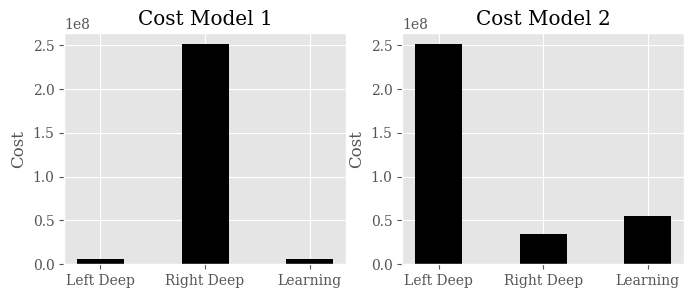
\includegraphics[width=\columnwidth]{figs/teaser.png}
    \caption{\small Query 12b from the Join Order Benchmark with 2 different cost models. Cost model 1 models a hash-join operator with a linear cost in the size of the input relations, and Cost model 2 models re-use of already built hash tables. A learning-based strategy is competitive with the dominant heuristic in both models. \label{teaser}}
\end{figure}

If we wanted to avoid the pitfalls of such pruning heuristics, we could exhaustively enumerate all join plans including ``bushy'' join trees and cartesian products.
The principle of optimality leads to a dynamic programming algorithm that builds a lookup table of optimal subplans and their costs. 
As join optimization is known to be super-exponential in the number of tables, exhaustive methods scale very poorly.
Suppose, we only partially populated this lookup table.
Would it be possible to use machine learning to \emph{predict} the missing values?
Using machine learning is particularly compelling idea if a single model could apply to all queries in a workload and share learned cost structure across planning instances.

Algorithmically, this concept of approximate dynamic programming is exactly the focus of the Artificial Intelligence field of reinforcement learning (RL)~\cite{sutton1998reinforcement}. RL algorithms use sampling and statistical machine learning to estimate the long-term benefit of decisions.
In the join optimization context, this corresponds to a regression problem between the decision to join a particular set of relations and the cost-to-go function.
Since this regression problem can be very non-linear, we need a sufficiently rich class of functions, like neural networks, to parametrize the model.
With this formulation, we can apply standard RL algorithms, similar to the ones used to play Atari Games or the game of Go.
Going back to Figure \ref{teaser}, we train an RL model on 80 randomly selected queries from the Join Order benchmark and use the learned model to optimize the same query. The RL solution is competitive with the best heuristic in both cost models.

This learning-based approach gives us a new design space for query optimization.
Rather than the standard tuning parameters of a query optimizer, we now have to control what training data the model sees and how that data is featurized.
The model naturally shares query processing information across planning instances with the neural network parameters.
We can also vary the features used to represent the subplans, to allow the network to allow plans to be robust to available resources and cost estimation inaccuracies.
We can also augment the model with observations of actual query execution times and naturally incorporate feedback.

In short, (deep) reinforcement learning provides a new algorithmic perspective for thinking about join enumeration. 
Our system, called \sys, is built on Apache Calcite and we present extensive results on the join order benchmark.
We show \sys optimizes plans well across many different cost models for a relatively modest set of training queries.
Admittedly, this raises a new set of problems including overfitting and avoiding high-variance plans.
We hope that \sys is the first step in an entire spectrum of techniques between pure Deep RL and classical query optimization.

 

